\subsection{Full Model}
The final model for the TFETI method without Dirichlet preconditioner is given by the following formula
% \begin{equation}
% \begin{aligned}
% &\verb!time ~ timeAsmK + timeFactK + timeAsmGGTT!\\
% &\verb!       + iterNum*(timeActKT + timeActGGTT + timeActPrec),!
% \end{aligned}
% \label{eq:finalTFETI}
% \end{equation}

\begin{equation}
\begin{aligned}
t_e \approx\; &t_{K|asm} + t_{K|fact} + t_{GG^T|asm|T}\\ &+ iter \cdot (t_{K|act|T} + t_{GG^T|act|T} + t_{Prec|act}),
\end{aligned}
\label{eq:finalTFETI}
\end{equation}
where $t_e$ is the estimated run-time of ESPRESO, $iter$ is the estimated number of PPCG iterations  and $t_{Prec|act}$ equals $t_{Lump|act} + t_{GG^T|act|T}$ if Lumped preconditioner is used or 0 if there is no preconditioner.


When using Dirichlet preconditioner which requires extra preprocessing time the formula must be modified to

\begin{equation}
\begin{aligned}
t_e \approx\;  &t_{K|asm} + t_{K|fact} +  t_{GG^T|asm|T} +  t_{Dir|asm}\\ &+ iter\cdot(t_{K|act} + 2t_{GG^T|act|T} + t_{Dir|act})  
\end{aligned}
\label{eq:finalTFETIDirichlet}
\end{equation}
For HTFETI method both formulas remain very similar, only $t_{GG^T|asm|T}$, t$_{GG^T|act|T}$ and $t_{K|act|T}$ will be replaced with $t_{GG^T|asm|HT}$, t$_{GG^T|act|HT}$, $t_{K|act|HT}$. In case of the HTFETI method an extra preprocessing is also necessary $t_{F_0|asm}$, t$_{S\alpha|asm}$. 


So, the model for HTFETI without preconditioner or using Lumped preconditioner
will be modified as

\begin{equation}
\begin{aligned}
t_e \approx\; &t_{F|asm} + t_{S_\alpha|asm} + t_{K|asm} + t_{K|fact} + t_{GG^T|asm|HT} \\
&+ iter \cdot (t_{K|act|HT} + t_{GG^T|act|HT} + t_{Prec|act})
\end{aligned}
\label{eq:finalHTFETI}
\end{equation}
and the model for HTFETI with Dirichlet preconditioner as

\begin{equation}
\begin{aligned}
t_e \approx\; &t_{F|asm} + t_{S_\alpha|asm} + t_{K|asm} + t_{K|fact} + t_{GG^T|asm|HT}  + t_{Dir|asm}\\
&+ iter \cdot (t_{K|act|HT} + 2t_{GG^T|act|HT} + t_{Dir|act})
\end{aligned}
\label{eq:finalHTFETIDirichlet}
\end{equation}


\section{Model Validation}
The final model was validated using RMSE\cite{rmse}, sMAPE\cite{smape} and finally
by the simple comparison of the difference between measured run-time with estimated 
optimal settings and the manually found optimal run-time.

We can see the whole fit of the final TFETI and HTFETI model in Fig. \ref{fig:finalTFETIModel} and \ref{fig:finalHTFETIModel}, respectively.

\begin{figure}[htb]
\centering
\begin{minipage}{0.3\textwidth}
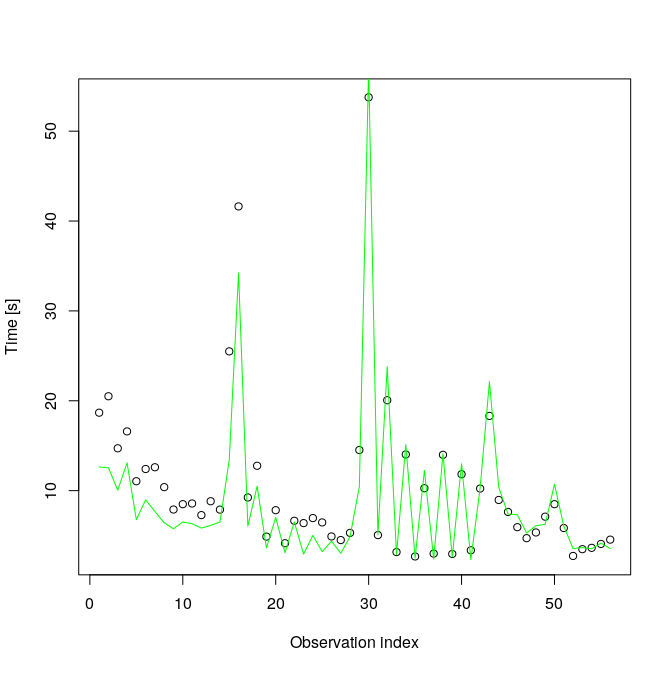
\includegraphics[width=\textwidth]{figures/tfeti-none.png}
\end{minipage}
\begin{minipage}{0.3\textwidth}
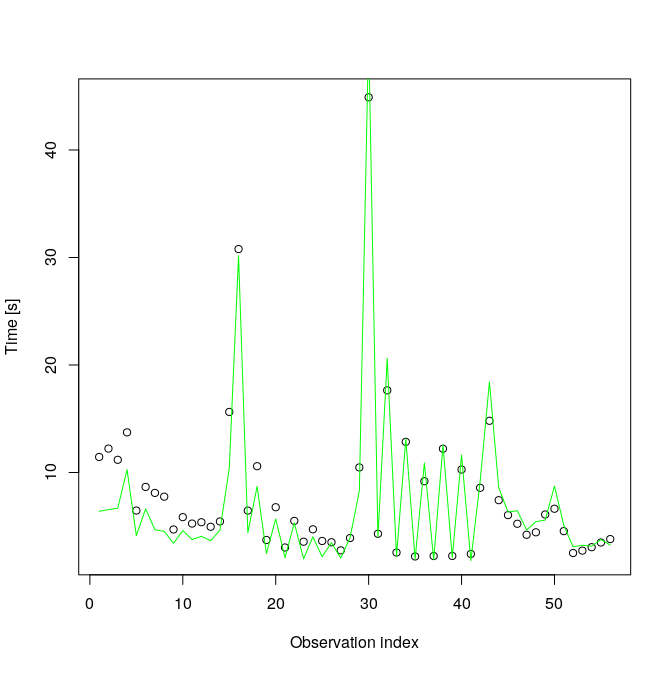
\includegraphics[width=\textwidth]{figures/tfeti-lumped.png}
\end{minipage}
\begin{minipage}{0.3\textwidth}
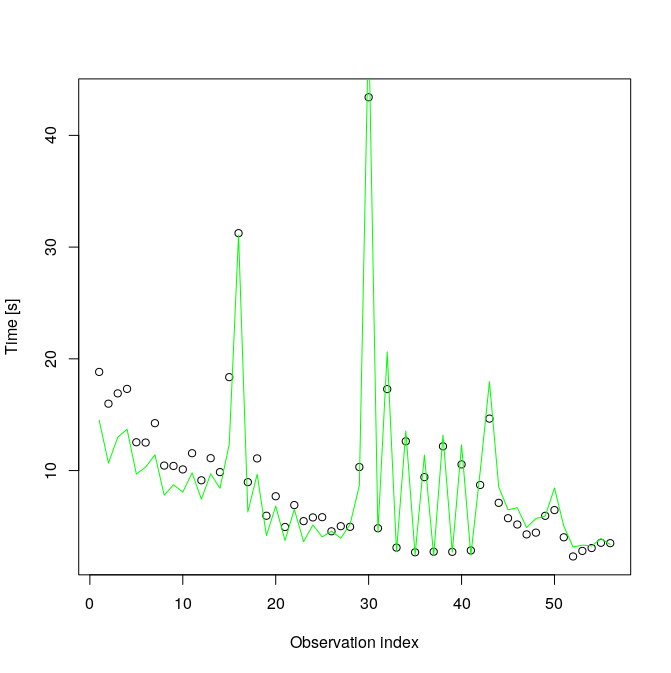
\includegraphics[width=\textwidth]{figures/tfeti-dirichlet.png}
\end{minipage}
\caption{Total FETI model fit with: no preconditioner (left), Lumped precondition (middle) and Dirichlet preconditioner (right).}
\label{fig:finalTFETIModel}
\end{figure}

The estimations of the optimal settings and their comparison with real optima can be seen in the Tab. \ref{tab:finalModelTest}, where \textit{Predicted time} is the 
minimal run-time estimated by the model together with the corresponding \textit{Predicted settings}. \textit{Measured time from predicted settings} is the 
manually measured run-time using the predicted settings from the model estimation. 
\textit{Optimal time} is then the manually found optima and \textit{Optimal settings} 
are the corresponding settings to the optimal time. Finally, \textit{Prediction error} is the difference between the measured time from predicted settings and the 
optimal time, i.e. the difference users would get if they were using the model for their computations.

\begin{table}[!htb]
\centering
\begin{tabular}{lcccccc}
\multicolumn{1}{c}{} & \multicolumn{6}{c}{\textbf{1728000 DOFs}} \\ \cline{2-7} 
\multicolumn{1}{l|}{} & \multicolumn{3}{c}{\textbf{TFETI}} & \multicolumn{3}{c|}{\textbf{HTFETI}} \\ \hline
\multicolumn{1}{|r|}{\textbf{Preconditioner}} & \multicolumn{1}{c|}{\textbf{None}} & \multicolumn{1}{c|}{\textbf{Lumped}} & \multicolumn{1}{c|}{\textbf{Dirichlet}} & \multicolumn{1}{c|}{\textbf{None}} & \multicolumn{1}{c|}{\textbf{Lumped}} & \multicolumn{1}{c|}{\textbf{Dirichlet}} \\ \hline
\multicolumn{1}{|l|}{\begin{tabular}[c]{@{}l@{}}Predicted settings: \\ \# of compute nodes \\ \# of MPI processes per node\\ \# of Cilk threads per MPI p.\\ \# of domains per MPI rank \\ domain size {[}DOF{]}\end{tabular}} & \begin{tabular}[c]{@{}c@{}}4\\ 24\\ 1\\ 18\\ 1029\end{tabular} & \begin{tabular}[c]{@{}c@{}}4\\ 24\\ 1\\ 18\\  1029\end{tabular} & \multicolumn{1}{c|}{\begin{tabular}[c]{@{}c@{}}4\\ 8\\ 3\\ 48\\ 1029\end{tabular}} & \begin{tabular}[c]{@{}c@{}}16\\ 4\\ 6\\ 64\\ 375\end{tabular} & \begin{tabular}[c]{@{}c@{}}16\\ 24\\ 1\\ 12\\ 375\end{tabular} & \multicolumn{1}{c|}{\begin{tabular}[c]{@{}c@{}}16\\ 4\\ 6\\ 64\\ 375\end{tabular}} \\ \hline
\multicolumn{1}{|l|}{Predicted time {[}s{]}} & 2.32 & 1.8 & \multicolumn{1}{c|}{2.39} & 0.78 & 0.66 & \multicolumn{1}{c|}{0.76} \\ \hline
\multicolumn{1}{|l|}{\begin{tabular}[c]{@{}l@{}}Measured time from \\ predicted settings {[}s{]}\end{tabular}} & 3.36 & 2.42 & \multicolumn{1}{c|}{2.74} & 0.77 & 1.05 & \multicolumn{1}{c|}{0.54} \\ \hline
\multicolumn{1}{|l|}{\begin{tabular}[c]{@{}l@{}}Optimal settings:\\ \# of compute nodes \\ \# of MPI processes per node\\ \# of Cilk threads per MPI p.\\ \# of domains per MPI rank \\ domain size {[}DOF{]}\end{tabular}} & \begin{tabular}[c]{@{}c@{}}4\\ 6\\ 4\\ 64\\ 1029\end{tabular} & \begin{tabular}[c]{@{}c@{}}4\\ 6\\ 4\\ 64\\ 1029\end{tabular} & \multicolumn{1}{c|}{\begin{tabular}[c]{@{}c@{}}16\\ 4\\ 6\\ 64\\ 375\end{tabular}} & \begin{tabular}[c]{@{}c@{}}16\\ 4\\ 6\\ 64\\ 375\end{tabular} & \begin{tabular}[c]{@{}c@{}}16\\ 4\\ 6\\ 64\\ 375\end{tabular} & \multicolumn{1}{c|}{\begin{tabular}[c]{@{}c@{}}16\\ 4\\ 6\\ 64\\ 375\end{tabular}} \\ \hline
\multicolumn{1}{|l|}{Optimal time {[}s{]}} & 2.68 & 2.19 & \multicolumn{1}{c|}{2.31} & 0.77 & 0.53 & \multicolumn{1}{c|}{0.54} \\ \hline
\multicolumn{1}{|l|}{RMSE} & 3.14 & 2.13 & \multicolumn{1}{c|}{2.21} & 4 & 1.37 & \multicolumn{1}{c|}{1.49} \\ \hline
\multicolumn{1}{|l|}{sMAPE} & 0.23 & 0.23 & \multicolumn{1}{c|}{0.18} & 0.43 & 0.27 & \multicolumn{1}{c|}{0.24} \\ \hline
\multicolumn{1}{|l|}{Prediction error {[}s{]}} & 0.69 & 0.23 & \multicolumn{1}{c|}{0.42} & 0 & 0.51 & \multicolumn{1}{c|}{0} \\ \hline
\end{tabular}
\caption{Evaluation of the final model prediction quality}
\label{tab:finalModelTest}
\end{table}

\begin{figure}[htb]
\centering
\begin{minipage}{0.3\textwidth}
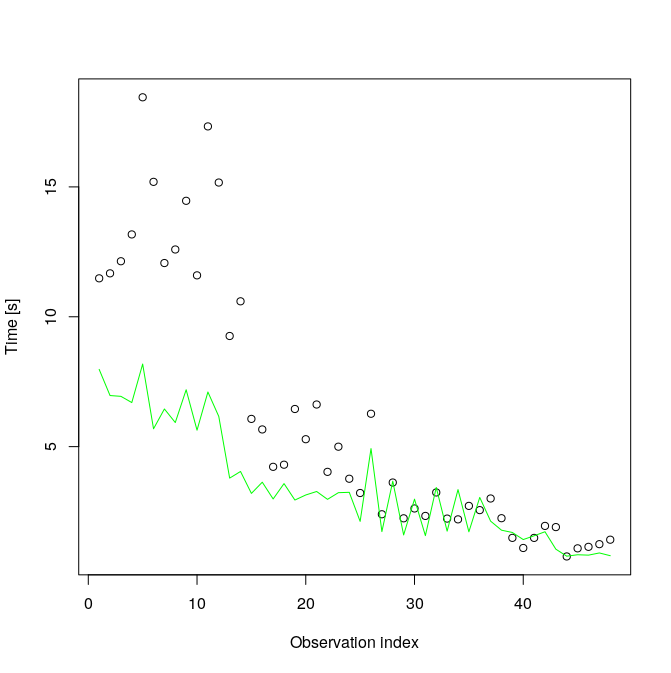
\includegraphics[width=\textwidth]{figures/htfeti-none.png}
\end{minipage}
\begin{minipage}{0.3\textwidth}
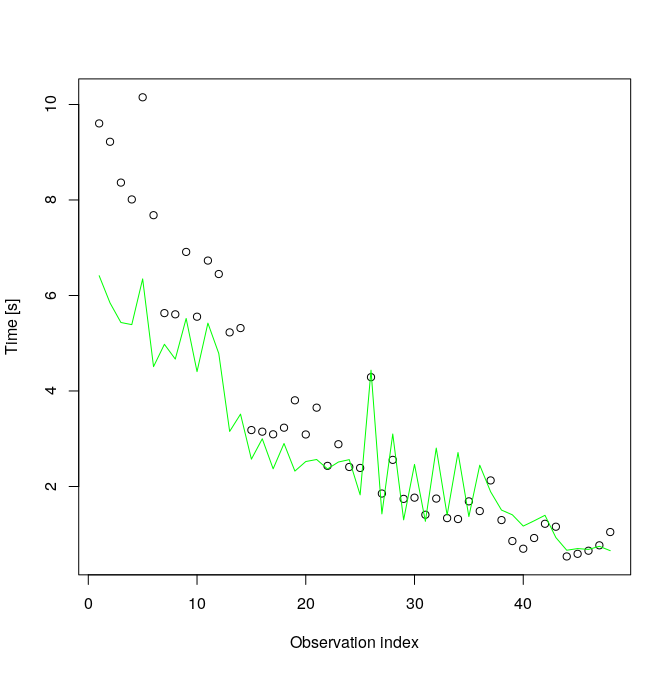
\includegraphics[width=\textwidth]{figures/htfeti-lumped.png}
\end{minipage}
\begin{minipage}{0.3\textwidth}
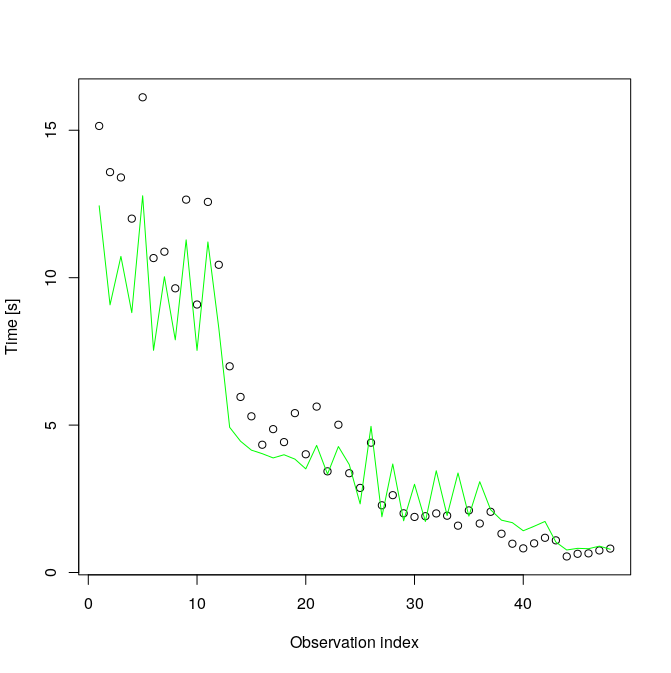
\includegraphics[width=\textwidth]{figures/htfeti-dirichlet.png}
\end{minipage}
\caption{Hybrid Total FETI model fit with: no preconditioner (left), Lumped precondition (middle) and Dirichlet preconditioner (right).}
\label{fig:finalHTFETIModel}
\end{figure}